\documentclass[11pt,a4paper]{article}
\usepackage[T1]{fontenc}
\usepackage[utf8]{inputenc}
\usepackage[margin=2.5cm]{geometry}
\usepackage{amsmath,booktabs,graphicx}
\usepackage[colorlinks=true,allcolors=blue]{hyperref}

\title{Chess Rating Estimation --- Progress Notes}
\author{}
\date{\today}

\begin{document}
\maketitle

\section{Setting}
Classify the rating bin of a game from the game itself (moves, clocks, opening,
time control). One row per game, label \texttt{elo\_bin} from the average Elo of
both players. Data: Lichess standard rated rapid games, April--June 2017.
Model: XGBoost. Headline metric: accuracy; per-bin accuracy and the confusion
matrix as diagnostics.

\section{Sampling}
34.6M games read, 7.64M rapid, 4.53M eligible. Filters: rated, rapid
($480 \le \text{base} + 40\cdot\text{inc} \le 1499$), no bots, no abandoned or
rules-infraction games, $|\Delta\text{Elo}| \le 100$, at least 20 half-moves.
Stratified reservoir sampling over 9 bins of 200 Elo, cap 50\,000 per bin
(333\,478 games; 13\,h single-threaded).

\begin{center}
\begin{tabular}{lrrr}
\toprule
Bin & Kept & Eligible & Retention \\
\midrule
$<800$        & 47      & 47        & 100\,\% \\
$[800,1000)$  & 22\,340 & 22\,340   & 100\,\% \\
$[1000,1200)$ & 50\,000 & 232\,583  & 21.5\,\% \\
$[1200,1400)$ & 50\,000 & 762\,977  & 6.5\,\% \\
$[1400,1600)$ & 50\,000 & 1\,383\,785 & 3.6\,\% \\
$[1600,1800)$ & 50\,000 & 1\,329\,333 & 3.8\,\% \\
$[1800,2000)$ & 50\,000 & 662\,901  & 7.5\,\% \\
$[2000,2200)$ & 50\,000 & 121\,233  & 41.2\,\% \\
$\ge 2200$    & 11\,091 & 11\,091   & 100\,\% \\
\bottomrule
\end{tabular}
\end{center}

The tails are exhausted and stay below the target. For modelling the bins are
merged to 7 classes: $<1000$ (from $<800$ and $[800,1000)$) and $\ge 2000$
(from $[2000,2200)$ and $\ge 2200$).

\section{Train/test split}
The label is mostly a property of the player, so train and test must be
player-disjoint; otherwise the model can recognise players by their play. A game
whose players land on different sides is dropped.

\begin{itemize}
  \item 91\,620 players; 31\% have one game, but players with $\ge 10$ games hold
        68\% of all player slots. 39\% of players span more than one bin.
  \item Player graph (edge = played each other): 97.3\% of players and 99.5\% of
        games are in one connected component, so a split cannot follow
        components (Fig.~\ref{fig:graph}).
  \item With independent assignment and fractions $p_i$, a game survives with
        probability $\sum_i p_i^2$ and lands in split $i$ with probability $p_i^2$.
        An 80/10/10 player split gives a 97/1.5/1.5 game split and loses 34\%.
        Graph partitioning could lose less; not measured.
\end{itemize}

\begin{figure}[h]
  \centering
  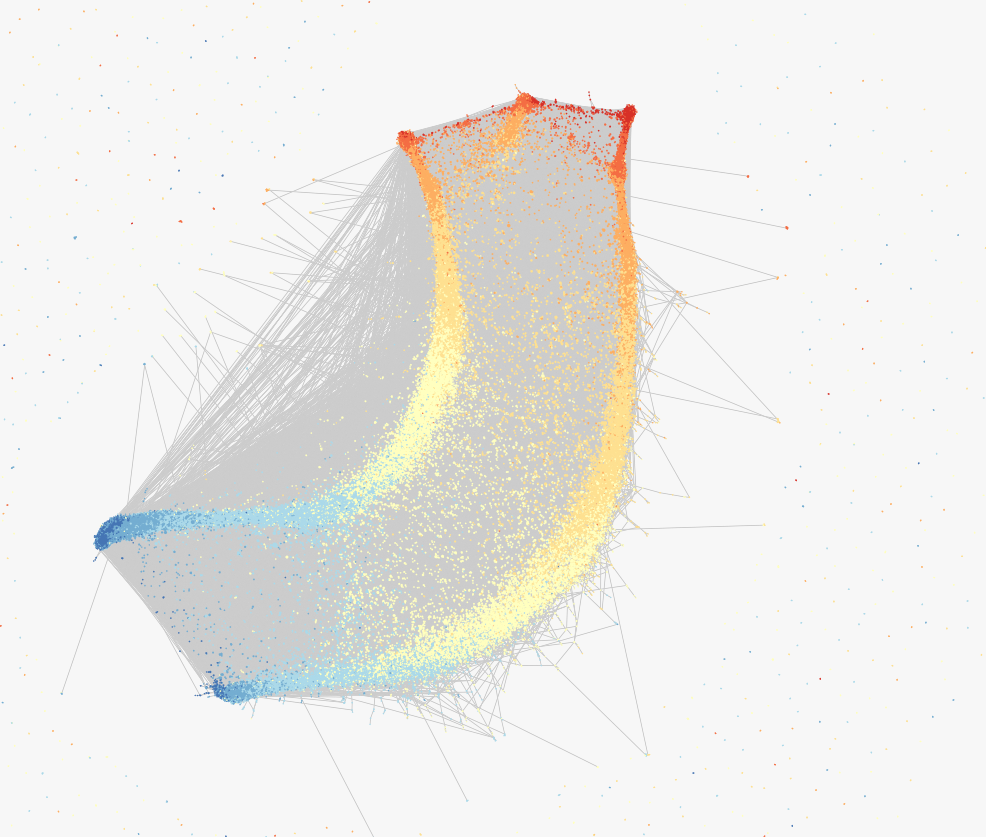
\includegraphics[width=0.45\linewidth]{images/PlayerGraph.png}
  \caption{Player graph, nodes coloured by rating bin.}
  \label{fig:graph}
\end{figure}

\textbf{Test size.} $SE \le 0.5/\sqrt{n}$. About 10\,000 test games give
$\pm 1.0$\,pp at most (95\%, independent). Games of one player are correlated:
with $\bar m \approx 2.5$ test games per player and an assumed within-player
error correlation $\rho = 0.1$--$0.5$, the interval widens by
$\sqrt{1+(\bar m-1)\rho} \approx 1.07$--$1.32$, so roughly $\pm 1.3$\,pp.
This is approximate, since a game has two players. Test fraction
$p_\text{test}^2 \cdot 333\,478 \approx 10\,000$ gives $p_\text{test} \approx 0.173$.

\textbf{Result.} Independent assignment within 9 strata (quantiles of player
mean Elo), seed 42, train/test = 0.827/0.173.

\begin{center}
\begin{tabular}{lrrr}
\toprule
 & Games & Players & Share of kept \\
\midrule
Train & 229\,402 & 71\,198 & 96.0\% \\
Test  &   9\,666 &  7\,688 &  4.0\% \\
\midrule
Dropped & 94\,410 (28.3\%) & & \\
\bottomrule
\end{tabular}
\end{center}

Retention 71.7\% (predicted 71.4\%). Disjointness check passes. Test ratings are
7--35 Elo lower than train across the deciles (mean 1563 vs.\ 1578; KS 0.023).

Games per class after merging:
\begin{center}
\begin{tabular}{lrrrrrrr}
\toprule
 & $<$1000 & 1000--1200 & 1200--1400 & 1400--1600 & 1600--1800 & 1800--2000 & $\ge$2000 \\
\midrule
Train & 14\,851 & 34\,545 & 34\,514 & 34\,430 & 34\,389 & 33\,862 & 42\,811 \\
Test  & 778 & 1\,449 & 1\,421 & 1\,417 & 1\,416 & 1\,576 & 1\,609 \\
\bottomrule
\end{tabular}
\end{center}

\textbf{Baselines (test).} Majority class ($\ge 2000$): 16.6\%. Uniform: 14.3\%.
Every model accuracy is reported next to these.

\textbf{Validation.} No fixed validation set (it would pay the $p_i^2$ cost again).
Hyperparameters use 5-fold CV inside train with folds assigned by player. A game
is a validation row of fold $k$ if both players are in $k$, a fit row if neither
is, and is used for fitting in the other folds if its players are in different
folds. Each validation fold then holds only about 1/25 of the games ($\approx$9\,000).

\textbf{Rejected.}
\begin{itemize}
  \item Temporal split: same players on both sides, leaks the label.
  \item Random 80/10/10 player split: see above.
  \item Split the eligible pool first, then sample: protects the tails, but means
        redoing the 13\,h sampling run.
\end{itemize}

\section{Features}
Excluded (label or identity): \texttt{white\_elo}, \texttt{black\_elo},
\texttt{avg\_elo}, \texttt{rating\_diff}, \texttt{white}, \texttt{black},
\texttt{game\_id}, \texttt{utc\_date}, \texttt{utc\_time}, \texttt{split}.
Current inputs: result, termination, half-moves, moves, clocks,
\texttt{opening\_family}, \texttt{tc\_base}, \texttt{tc\_increment}.
Anything fitted on data (e.g.\ opening target encoding) is fitted on training
rows only, inside each CV fold.

\textbf{Stockfish (in progress).} Engine features (centipawn loss, blunders,
best-move agreement) for all train/test games, run on a rented machine with a
hard cap of \$20. Calibration on 350 games (50 per bin), depths 15/18/20 and
MultiPV 1--3: per-game ACPL vs.\ Elo has Spearman $\rho \approx -0.52$ for every
configuration, with overlapping 95\% CIs, so no measurable gain from more depth
or MultiPV. Depth 15, MultiPV 1 is the leading candidate (est.\ \$5, unverified
cloud price); final choice open.

\section{Open}
\begin{itemize}
  \item Engine depth/MultiPV decision and the full remote run.
  \item Remaining PGN features (clock usage, development, castling).
  \item Class weights for the sparse $<1000$ class.
  \item CV fold construction.
  \item Baseline XGBoost, then lift from engine features.
\end{itemize}

\end{document}
